\documentclass[12pt,a4paper]{report}

\usepackage{bookman}
\usepackage{ngerman}
\usepackage[T1]{fontenc}
\usepackage[utf8]{inputenc}
\usepackage{graphicx}
\usepackage{tabularx}
\usepackage[left=2cm,right=2cm,top=2cm,bottom=2cm]{geometry}
\usepackage{custompkg}

\begin{document}
	\bslinespacing{1.5}
	
	\Huge Gruppe 47
	\hspace{2cm}
	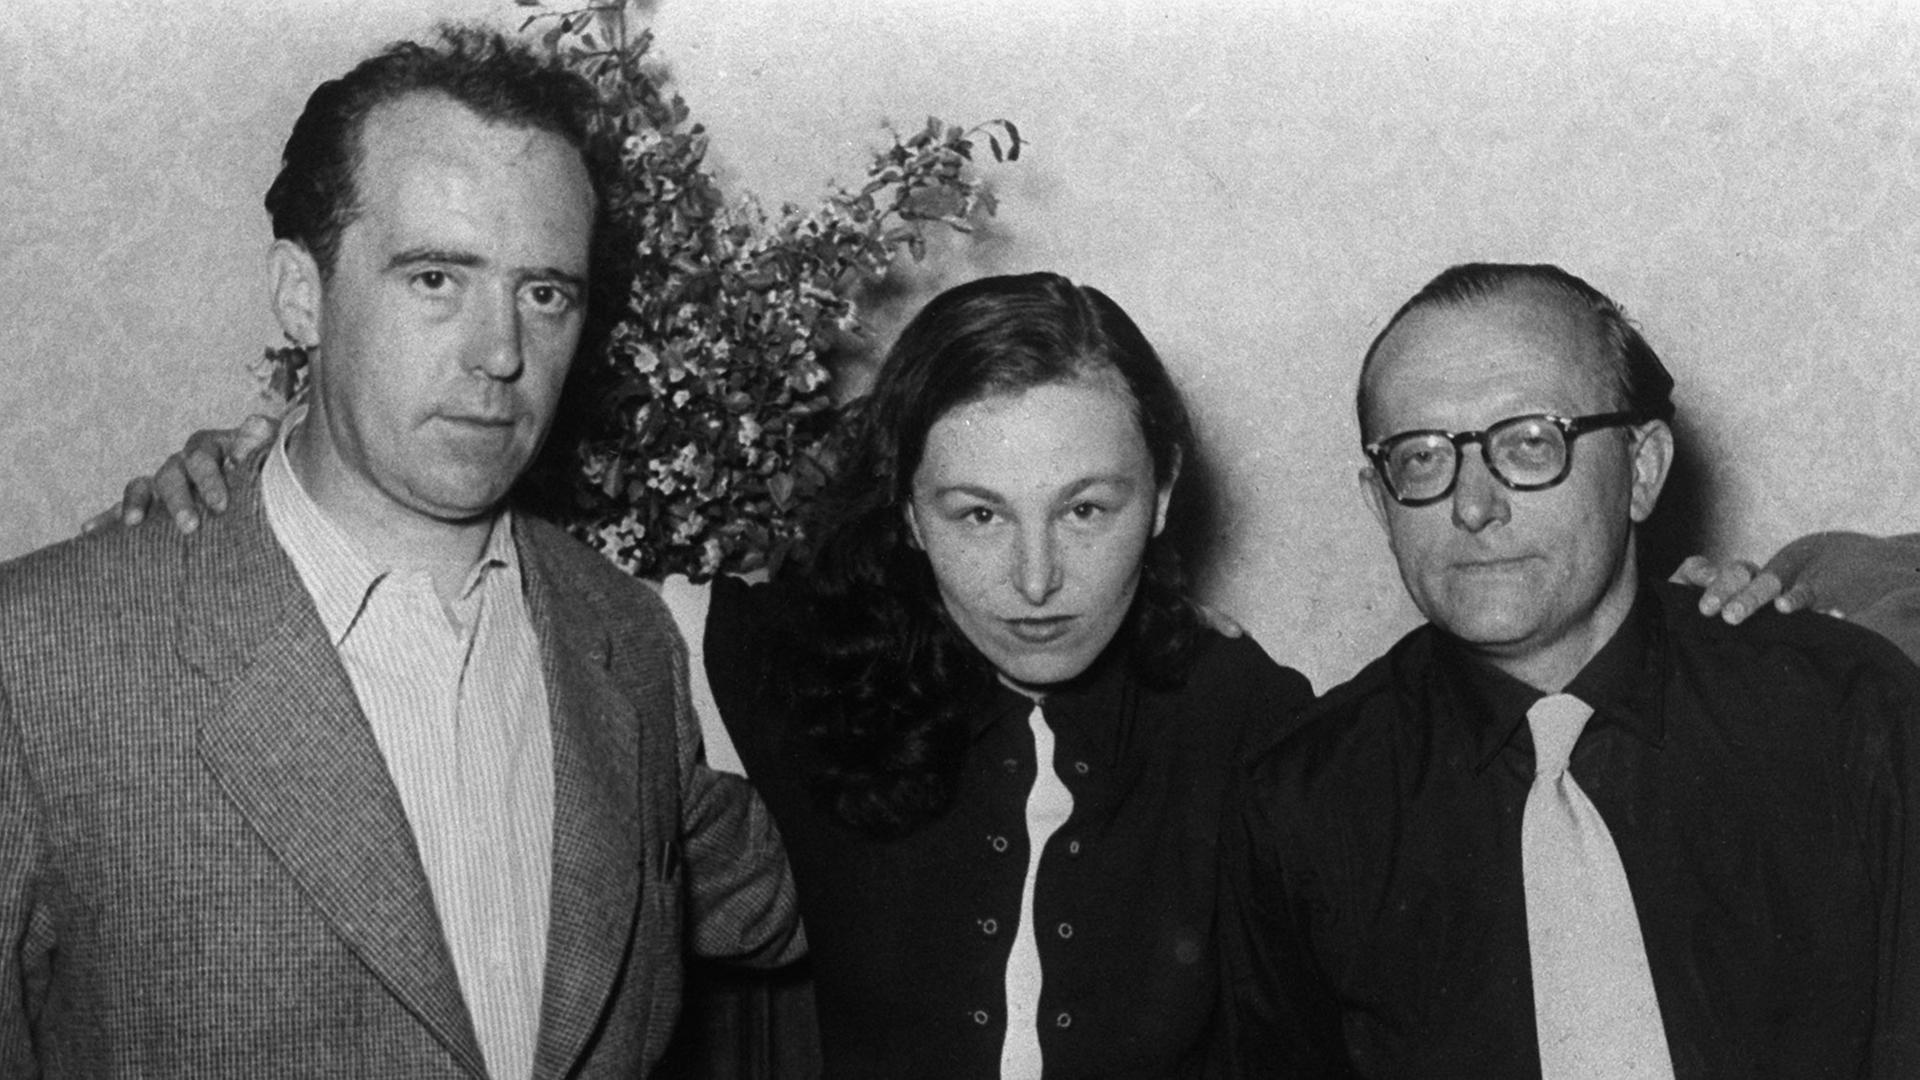
\includegraphics[width=8cm]{IMG_1745.jpeg}

	\vspace{1cm}
	\normalsize
	
	\paragraph{Generelles}
	
	\begin{itemize}
		\item Deutschsprachiges Schriftstellertreffen
		\item Gegründet 1947 von Hans Werner Richter
		\item Das Treffen diente der gegenseitigen Kritik vorgelesener Texte und der Förderung junger, unbekannter Autoren.
	\end{itemize}
	
	\paragraph{Mitglieder} \mbox{} \\\\
	\begin{tabularx}{\textwidth}{|X|X|X|}
		\hline
		\textbf{Mitglied} & \textbf{Funktion} & \textbf{erste Teilnahme} \\
		\hline
		Hans Magnus Enzensberger & Autor & 1955 \\
		
	\end{tabularx}
	

	
\end{document}